\documentclass[french]{article}
\usepackage[utf8]{inputenc}
\usepackage[T1]{fontenc}

\usepackage{natbib}
\usepackage[vmargin=4cm,left=4cm,right=4cm]{geometry}

\usepackage{amsmath}

\usepackage{babel}

\usepackage{graphicx}
\usepackage{caption} 
\captionsetup{justification=centering}
\usepackage{subcaption}
% \usepackage{hyperref}
\usepackage[hidelinks]{hyperref}

% ################################
% Package pour incorporer du code
\usepackage{xcolor,colortbl}
\usepackage{listings}

\definecolor{codegreen}{rgb}{0,0.6,0}
\definecolor{codegray}{rgb}{0.5,0.5,0.5}
\definecolor{backcolour}{rgb}{0.96,0.96,0.96}

\lstdefinestyle{mystyle}{
    literate=
  {²}{{\textsuperscript{2}}}1
  {⁴}{{\textsuperscript{4}}}1
  {⁶}{{\textsuperscript{6}}}1
  {⁸}{{\textsuperscript{8}}}1
  {€}{{\euro{}}}1
  {é}{{\'e}}1
  {è}{{\`{e}}}1
  {ê}{{\^{e}}}1
  {ë}{{\¨{e}}}1
  {É}{{\'{E}}}1
  {Ê}{{\^{E}}}1
  {û}{{\^{u}}}1
  {ù}{{\`{u}}}1
  {â}{{\^{a}}}1
  {à}{{\`{a}}}1
  {á}{{\'{a}}}1
  {ã}{{\~{a}}}1
  {Á}{{\'{A}}}1
  {Â}{{\^{A}}}1
  {Ã}{{\~{A}}}1
  {ç}{{\c{c}}}1
  {Ç}{{\c{C}}}1
  {õ}{{\~{o}}}1
  {ó}{{\'{o}}}1
  {ô}{{\^{o}}}1
  {Õ}{{\~{O}}}1
  {Ó}{{\'{O}}}1
  {Ô}{{\^{O}}}1
  {î}{{\^{i}}}1
  {Î}{{\^{I}}}1
  {í}{{\'{i}}}1
  {Í}{{\~{Í}}}1,
    backgroundcolor=\color{backcolour},   
    commentstyle=\color{codegreen},
    keywordstyle=\color{blue},
    numberstyle=\color{codegray},
    stringstyle=\color{orange},
    basicstyle=\ttfamily\small, % \footnotesize,
    breakatwhitespace=false,         
    breaklines=true,                 
    captionpos=b,                    
    keepspaces=true,                 
    numbers=left,                    
    numbersep=10pt,                  
    showspaces=false,                
    showstringspaces=false,
    showtabs=false,
}

\lstset{style=mystyle}

%##################################


\begin{document}

%###############################################
\begin{titlepage}

\newcommand{\HRule}{\rule{\linewidth}{0.5mm}} % Defines a new command for the horizontal lines, change thickness here

\center % Center everything on the page
 
%----------------------------------------------------------------------------------------
%	Section Titre
%----------------------------------------------------------------------------------------
\HRule \\[0.4cm]
\vspace{1cm}
{ \huge \bfseries Premier modèle KNN}\\ % Title of your document
\vspace{1cm}
\HRule \\[1cm]
 
%----------------------------------------------------------------------------------------
%	Section auteur
%----------------------------------------------------------------------------------------
\vspace{1cm}

\Large \today

\vspace{3cm}

\begin{minipage}{0.4\textwidth}
\begin{center}
\Large \textbf{Auteurs :}\\
\vspace{0.5cm}
Fabio \textsc{Cassiano}
\end{center}
\end{minipage}

\vspace{5cm}

\begin{figure}[!ht]
    %\hspace*{-0.5cm}
	
\includegraphics[height=0.1\columnwidth]{images/logo/logo_simplon.png}
	\hspace*{0.5cm}
	
\includegraphics[height=0.12\columnwidth]{images/logo/logo_Isen.png}
	\hspace*{0.5cm}
	
\includegraphics[height=0.1\columnwidth]{images/logo/logo_microsoft.jpg}
\end{figure}

\vfill

\end{titlepage}

\newpage

\tableofcontents

\vspace{1cm}

\listoffigures

\newpage


\section{Questionnaire de personnalité}

Un test de personnalité a été mis au point sous python, afin de déterminer la personnalité des participants. Chaque personne doit répondre à 10 questions afin d'obtenir un score, sur lequel sera basé la mise en relation avec une personnalité.\\

Notre objectif ici est d'essayer de prédire la personnalité d'une personne en fonction de ses réponses aux différentes questions, en utilisant un modèle \textit{K-nearest neighboors} (KNN) sans estimer de score. Pour ce faire la première étape est de se constituer un jeu de données. Plusieurs personnes ont ainsi réalisé les questionnaires 10 fois consécutives générant ainsi un fichier \textit{csv} par participant.

\section{Création du jeu de données (DataSet)}

La création du DataSet se fait en réalisant la concaténation des différents fichier \textit{csv}, afin d'avoir un DataSet suffisament conséquent. Cette étape est réalisé à l'aide de la fonction \textit{create\_DataSet()}. Cette fonction parcours le dossier contenant tout les fichiers \textit{csv}, chacun d'entre eux est ensuite lu avec la fonction \textit{read\_csv()} du module \textbf{pandas}, le contenu est ajouté à la liste \textit{data\_list} qui est ensuite concaténé afin de renvoyer le DataSet (\textit{data}). 

\subsection{Code Python - \textit{create\_DataSet()}}

\begin{lstlisting}[language=Python]
def create_DataSet():
    file_list = os.listdir("./DataSet/")
    data_list = []
    for i in file_list:
        data_list.append(pd.read_csv("./DataSet/{}".format(i)))

    data = pd.concat(data_list)
    
    # # -------------------------------------------------------------
    # # ou pour enregistrer un nouveau csv :
    # data.to_csv( "data.csv", index=False, encoding='utf-8-sig')
    # # -------------------------------------------------------------

    return data
    
\end{lstlisting}

\section{Préparation du jeu de données}

La préparation du jeu de données est l'étape la plus importante, elle conditionne l'apprentissage du modèle ce qui impactera par conséquent les performances de ce dernier.\\
\noindent Afin de préparer le DataSet au mieux on réalise 3 étapes essentiel :
\begin{enumerate}
    \item Suppression des valeurs erronés.
    \item Remplacement des valeurs manquantes.
    \item Harmonisation des données.
\end{enumerate}

\subsection{Suppression des valeurs erronés}

Après avoir analysé le code du questionnaire de personnalité, il a été constaté que les utilisateurs ne sont pas limité dans leur réponse, c'est à dire qu'il peuvent répondre avec des valeurs non pris en compte dans le calcul du score. Il est donc essentiel, pour l'entraînement du modèle, de supprimer ces valeurs.\\

\noindent Pour ce faire, les valeurs valides ont été identifiées. Dans notre projet les valeurs sont les suivantes : \textit{"a", "b", "c", 1, 2, 3}. Toutes les autres valeurs sont donc identifier et remplacer pars des \textit{NaN}, afin d'être traiter dans l'étape suivante.

\subsection{Remplacement des valeurs manquantes}

Il a également été remarqué dans le code du questionnaire, que l'utilisateur peut laisser les champs vide, ce qui engendre des valeurs manquantes (\textit{NaN}) dans le jeu de données. Ces données doivent être traiter afin que le modèle puisse être entraîner. Pour ce faire deux solutions sont possibles :

\begin{itemize}
    \item Supprimer les observations contenant des données manquante.
    \item Remplacer les données par une autre valeur (moyenne, min, max, mode, etc..)
\end{itemize}

Dans notre cas, la suppression des données n'est pas envisageable au vu du nombre d'observation qui constitue notre jeu de données. Cela aurait pour impact de réduire fortement notre DataSet, ce qui empêcherait notre modèle d'être entraîner correctement.\\

\noindent Les données qui composent nos DataSet, sont des données de type qualitative. Il a donc été décidé de remplacer les données manquantes par le mode de chaque \textit{features}. Il aurait également été possible de remplacer les \textit{NaN}, par la valeur \textit{"b" ou 2}, qui sont les entrées qui n'impacte pas le calcul du score dans le code du questionnaire.

\subsection{Encodage des données}

La dernière étape a effectuer pour finir la préparation du DataSet est l'encodage des données, qui consiste à harmoniser les différentes \textit{features}. Pour ce faire plusieurs méthodes sont possible, il est possible d'encoder les données avec la fonction \textit{OneHotEncoder()}, de la librairie \textbf{Sklearn}, ce qui encodera les valeurs de manière binaires. Une autre possibilité étant de remplacer les valeurs \textit{"a", "b", "c"} par leurs correspondance numérique \textit{1, 2, 3}. Cette dernière solution est celle pour laquelle nous avons opté.\\

\noindent Enfin pour finir, le DataSet est divisé en un jeu d'entraînement (\textit{X\_train}) et un jeu de test (\textit{X\_train}), cela à l'aide de la fonction \textit{train\_test\_split()} de la librairie \textbf{sklearn}. Le DateSet est maintenant près pour entraîner notre modèle.

\section{Développement et entraînement d'un modèle KNN}

\subsection{Principe du KNN}

Le modèle que est développé ici, est celui des K plus proche voisin (KNN). Ce modèle a pour principe de calculer les distances entre une valeurs à tester avec les valeurs du jeu d'entraînement. Les k-distances les plus faible sont ensuite sélectionné, k étant le nombre de valeurs choisis lors de la création du modèle. La valeur testé est ensuite associé au label majoritaire présent dans les k plus faibles distances (voir Fig. \ref{fig:KNN_schema}.\\

\begin{figure}[!htbp]
    \centering
    \includegraphics[width=\textwidth]{images/KNN_schema.png}
    \caption{Représentation du principe du modèle de KNN - \textit{source : https://www.datacamp.com}.}
    \label{fig:KNN_schema}
\end{figure}

Les distances entre deux valeurs peuvent se calculer de différentes façon (voir Fig. \ref{fig:dist}). Dans notre étude nous nous intéresserons au méthode suivante : la distance euclidienne (eq. \ref{eq:eu}), la distance de manhattan (eq. \ref{eq:man}), ou encore la distance de minkowski (eq. \ref{eq:min}).\\

\begin{equation}\label{eq:eu}
    distance_{euclidienne} = \sqrt{\sum_{i=1}^{n} (x_{i} - y_{i})^{2}}\\
\end{equation}

\begin{equation}\label{eq:man}
    distance_{manhattan} = \sum_{i=1}^{n} |x_{i} - y_{i}|\\
\end{equation}

\begin{equation}\label{eq:min}
    distance_{minkowski} = \sqrt[\leftroot{}\uproot{}p]{\sum_{i=1}^{n} (x_{i} - y_{i})^{p}} 
\end{equation}

\begin{figure}[!htbp]
    \centering
    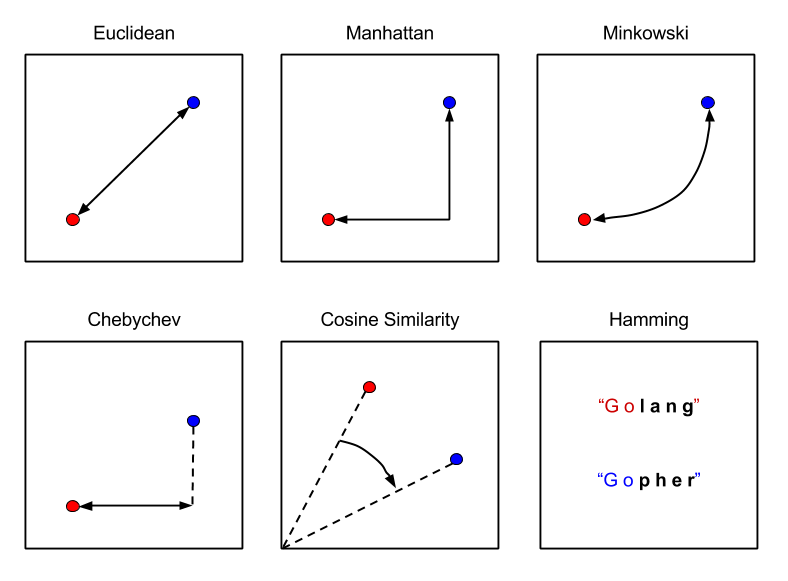
\includegraphics[width=\textwidth]{images/distance.png}
    \caption{Modélisation du calcul des différentes distances - \textit{source : \href{https://tuhinmukherjee74.medium.com/different-types-of-distances-used-in-machine-learning-explained-550e2979752c}{tuhinmukherjee74 sur medium}}.}
    \label{fig:dist}
\end{figure}

Dans cette partie nous entraînons deux modèles KNN, le premier étant celui que nous avons développé manuellement (from scratch), et le second est celui présent dans la librairie \textbf{sklearn}, le modèle \textit{KNeighborsClassifier()}.

\newpage

\subsection{KNN from scratch}

Le modèle KNN from scratch a été développé sous la forme d'une \textit{class}. Cette \textit{class \textbf{KNN()}} est composé de différentes méthodes permettant d'entraîner le modèle, mais égalment de calculer les distances, afin d'effectuer une prédiction, et même de calculer l'\textit{accuracy} de la prédiction. Ce modèle s'utilise avec des données de type \textit{array}, contenant uniquement des \textit{integer}.\\

\noindent Ce modèle s'utilise de la manière suivante :

\begin{enumerate}
    \item Initialisation d'une instance (création d'un modèle) : cela permet d'initialiser le modèle avec différentes propriétés.
    \item Entraîner le modèle avec le jeu d'entraînement (\textit{X\_train}), les labels correspondant (\textit{y\_label}) et la méthode de calcul de distance désirée (\textit{metric}).
    \item Prédiction des labels du jeu de test (\textit{X\_test}).
    \item Estimation de l'\textit{accuracy} du modèle en comparant les vrai labels du jeu test (\textit{y\_test}) à celles prédites.
\end{enumerate}

\subsubsection{Code Python - \textit{class} KNN()}

\begin{lstlisting}[language=Python]
class KNN:

    def __init__(self):
        self.__label_train = []
        self.__X_train = []
        self.__metric = 'euclidean'
        self.__p = []
        self.__label = []
        self.__confusion_matrix = []
        self.__format_model = {}

    
    def distance(self, **kwargs):
        '''
        distance permet de calculer la distance d'un échantillon par rapport aux autres.

        Paramètres
        ---------------------
        metric: {'Euclidean', 'Manhattan', 'Minkowski'}
            methode à utiliser pour calculer la distance 
        '''

        X_test = kwargs.get("X_test", None)

        if self.__metric.lower() == 'euclidean':
            if len(X_test) == 1:
                d = np.sqrt(np.sum((self.__X_train-X_test)**2, axis=1))
                return np.array(d)
            else:
                d = []
                for x in X_test:
                    d.append(np.sqrt(np.sum((self.__X_train-x)**2, axis=1)))
                return np.array(d)
        elif self.__metric.lower() == 'manhattan':
            if len(X_test) == 1:
                d = np.sqrt(np.sum(abs(self.__X_train-X_test), axis=1))
                return np.array(d)
            else:
                d = []
                for x in X_test:
                    d.append(np.sqrt(np.sum(abs(self.__X_train-x), axis=1)))
                return np.array(d)
        elif self.__metric.lower() == 'minkowski':
            if len(X_test) == 1:
                d = pow(np.sum(abs(self.__X_train-X_test)**self.__p, axis=1), 1/self.__p)
                return np.array(d)
            else:
                d = []
                for x in X_test:
                    d.append(pow(np.sum(abs(self.__X_train-x)**self.__p, axis=1), 1/self.__p))
                return np.array(d)
        else:
            raise ValueError(f"metric prend en uniquement comme valeur 'euclidean', 'manhattan', ou 'minkowski' (saisie {self.__metric})")


    def target_format(self, Y_train):
        self.__label = Y_train.sort_values().unique()

        cpt = 1
        for k in self.__label:
            self.__format_model[k] = cpt
            cpt +=1
        
        target_formated = Y_train.replace(self.__format_model).values

        return target_formated


    def train(self, X_train, label_train, **kwargs):
        self.__p = kwargs.get('p', 2)
        self.__metric = kwargs.get("metric", "euclidiean")
        self.__label_train = self.target_format(label_train) # Formatage des labels
        self.__X_train = X_train


    def prediction(self, X_test, k=5):
        d = self.distance(X_test = X_test)

        if d.ndim == 1:
            d = d.reshape(1,-1)

        # ind = np.argsort(d,axis=0)[:k,:] # k : nombre de voisin
        ind = np.argsort(d,axis=1)[:,:k] # k : nombre de voisin

        ppv = []
        for i in ind:
            ppv.append(self.__label_train[i]) # .mode()
        
        # ppv = list(map(list, zip(*ppv))) # transposé liste
        ppv = np.array(ppv)

        proba = []
        for i in range(1,3+1):
            proba.append(np.count_nonzero(ppv == i, axis=1)/k)

        proba = np.array(proba).T

        y_pred = np.argmax(proba, axis=1)+1

        return y_pred

    def accuracy(self, y_test, y_pred, **kwargs):
        
        y_test = y_test.replace(self.__format_model).values
        self.__confusion_matrix = confusion_matrix(y_test, y_pred)
        error_rate = (1 - np.trace(self.__confusion_matrix)/np.sum(self.__confusion_matrix))*100
        accuracy = 100-error_rate

        if kwargs.get('resume', False):
            self.resume(accuracy, error_rate)


        return accuracy, error_rate

    
    def resume(self, accuracy, error_rate):
        if not(accuracy):
            print("Le calcul de l'accuracy est nécessaire, utiliser la fonction d'instance pour la calculer")
        else:
    
            print("\n ======  Résumé des métrique  =====\n")
            print("----------------------")
            print("Matrice de confusion")
            print(self.__confusion_matrix)

            print("\n=======================")
            print(f"\nAccuracy : {accuracy}")
            print(f"\nTaux d'erreur : {error_rate}")
            print("----------------------")

            cpt = 0
            for l in self.__label:
                P = self.__confusion_matrix[cpt,cpt]/self.__confusion_matrix.sum(axis=0)[cpt]
                R = self.__confusion_matrix[cpt,cpt]/self.__confusion_matrix.sum(axis=1)[cpt]

                cpt += 1
                print(f"\nPrécision classe {l} : {P}")
                print(f"\nSensibilité classe {l} : {R}")
                print("----------------------")

            print("\n=======================\n")
    
\end{lstlisting}

\subsubsection{Résultats obtenus}

Afin d'estimer la valeur de k et la métrique les plus optimals pour notre application, l'accuracy a été calculer pour chaque métrique en faisant varier la valeur \textit{k} de 1 à 3O (voir Fig. \ref{fig:KNN_scratch}). D'après les résultats obtenus les paramètres les plus adaptés à notre application sont, la métrique de  \textit{manhattan}, et un \textit{k} de 3 ou 4.\\

\begin{figure}[!htbp]
    \centering
    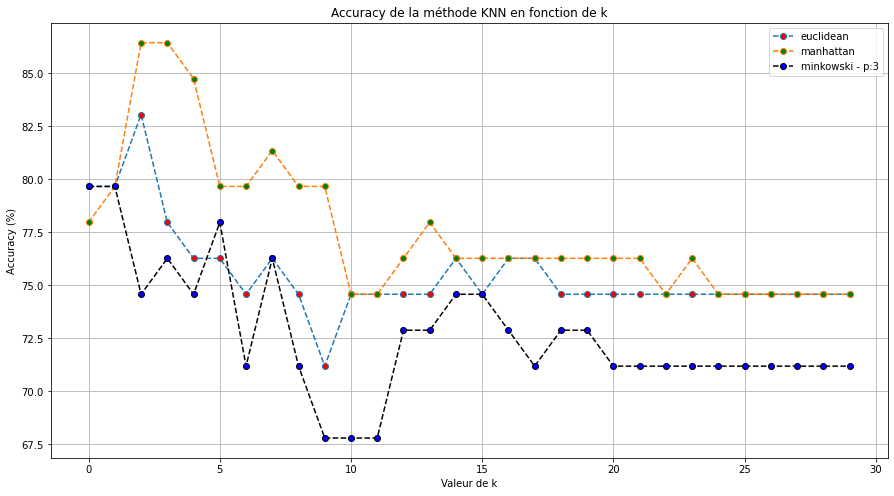
\includegraphics[width=\textwidth]{images/k_estimation.png}
    \caption{Évaluation de l'\textit{accuracy} du modèle from scratch en fonction du nombre de \textit{k}, pour les trois méthodes de calcul de distance.}
    \label{fig:KNN_scratch}
\end{figure}

Le paramètre \textit{p} pour la métrique \textit{minkowski}, a quant-à lui était étudié séparément afin de ne pas surcharger la représentation graphique. Cette étude a été réalisé avec un \textit{p} variant de 3 à 5. D'après les résultats obtenus la valeur \textit{p=3}, le modèle obtient de meilleur \textit{accuracy} (86\%) pour de k valant 5, 6 et 8.

\begin{figure}[!htbp]
    \centering
    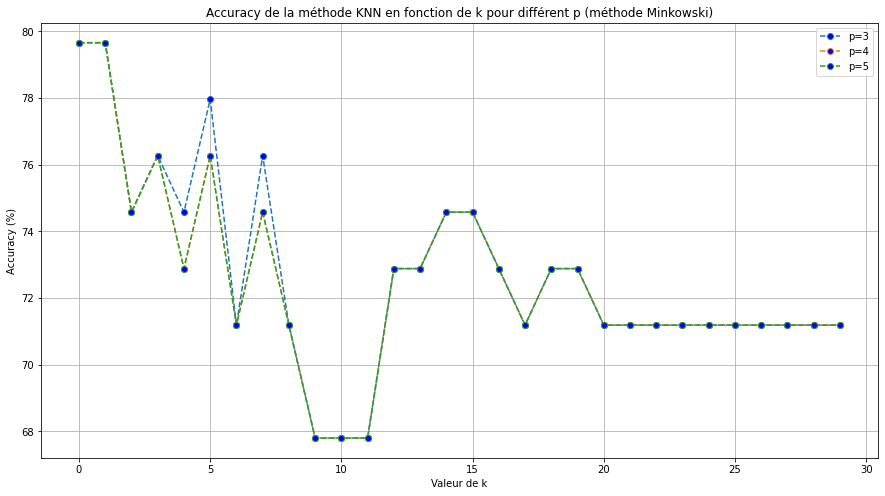
\includegraphics[width=\textwidth]{images/k_estimation_minkowki.png}
    \caption{Évaluation de l'\textit{accuracy} du modèle from scratch en fonction du nombre de \textit{k}, pour différentes valeurs de \textit{p}}
    \label{fig:KNN_min}
\end{figure}

\newpage

\subsection{KNN avec sklearn}

Les mêmes opérations, ainsi que les même jeu de données,  ont été utiliser pour entraîner le modèle KNN de \textbf{sklearn}. Dans un premier temps la détermination des meilleurs hyperparamètres a été réalisé visuellement comme pour le modèle from skratch. D'après les résultats obtenus paramètres permettant d'obtenir la meilleur \textit{accuracy} (83\%) sont, la métrique \textit{manhattan} et une valeur de k de 10.\\

\begin{figure}[!htbp]
    \centering
    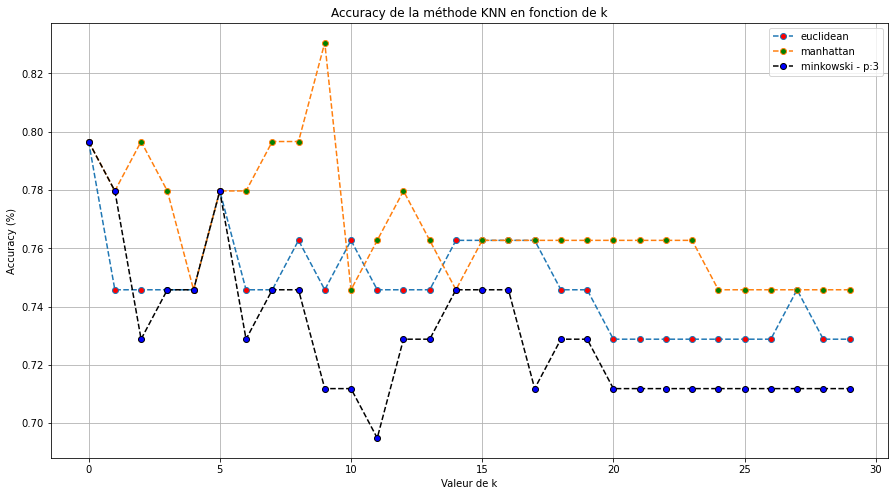
\includegraphics[width=\textwidth]{images/k_estimation_sklearn.png}
    \caption{Évaluation de l'\textit{accuracy} du modèle from scratch en fonction du nombre de \textit{k}, pour les trois méthodes de calcul de distance.}
    \label{fig:KNN_sklearn}
\end{figure}

Une autre façon d'estimer les meilleurs paramètres est d'utilisé la méthode de \textit{Grid-Search}, combiné avec la méthode \textit{K-fold}, grâce à la fonction \textit{GridSearchCV()}. Cela permet de tester les différentes combinaison possible et de réalisé les test sur K sous ensembles de notre jeu d'entraînement, afin d'éviter le sur-apprentissage. Le résultat obtenus par cette méthode est le même que le précèdent, la métrique \textit{manhattan} et un \textit{k=10}.


\section{Conclusion}

Les résultats obtenu par les modèles entraînés assez bon, avec une \textit{accuracy} dépassant les 80\% pour les deux modèles.\\

D'après notre étude il semblerait que l'on obtient les meilleurs performances de prédiction à partir du modèle KNN développé manuellement. Cela pourrait être expliqué par le fait que plusieurs paramètre du modèle KNN de \textbf{sklearn}, on été laissé par défaut.\\

Cependant pour ce cas d'étude il serait préférable de conservé la classification par le biais du score, pour ce faire il faudrait intervenir directement de le code du questionnaire afin de restreindre les réponses des utilisateurs.


\end{document}